\documentclass[iop]{emulateapj}
\usepackage{graphicx,hyperref,natbib}
\usepackage[usenames,dvipsnames,svgnames,table]{xcolor}
\graphicspath{{figures/}}
\usepackage{amsmath}
\newcommand{\blue}{\color{blue}}
\newcommand{\tam}{\color{blue}}
\newcommand{\tamcom}{\color{red}}
\newcommand{\red}{\color{red}}
\newcommand{\orange}{\color{orange}}
\newcommand{\purple}{\color{purple}}
\newcommand{\green}{\color{LimeGreen}}
\newcommand{\myemail}{samuelreay@gmail.com}
\newcommand{\runz}{\textsc{runz}}
\newcommand{\autoz}{\textsc{autoz}}

\newcommand{\marz}{\textsc{Marz}}

\shorttitle{Manual and Automatic Redshifting Software}
\shortauthors{S. R. Hinton}


\begin{document}

\title{\marz{}: Manual and Automatic Redshifting Software}

\author{S. R. Hinton, T. M. Davis, C. Lidman, K. Glazebrook, G. Lewis}
\affil{Department of Physics, The University of Queensland, Brisbane, QLD 4072, Australia}
\affil{ARC Centre of Excellence for All-sky Astrophysics (CAASTRO)}

\begin{abstract}
The Australian Dark Energy Survey (OzDES) is a 100-night spectroscopic survey underway on the Anglo-Australian Telescope using the fibre-fed 2-degree-field (2dF) spectrograph.  We have developed a new redshifting application \marz{} with greater usability, flexibility, and wider range of object types than the \runz{} software package previously used for redshifting spectra from 2dF. \marz{} is an open-source, client-based web-application which provides an intuitive interface and powerful automatic matching capabilities to consume FITs files generated from the AAOmega spectrograph and produce high quality spectroscopic measurements. Behind the scenes, a cross-correlation algorithm is used to match input spectra against a variety of stellar and galactic templates, and automatic matching performance for high quality spectra has increased from 57\% (\runz{}) to 94\% (\marz{}). Spectra not matched correctly by the automatic algorithm can be easily redshifted manually by cycling automatic results, manual template comparison, or marking spectral features.
\end{abstract}

\section{Introduction}


{\red introduce redshifting? introduce ozdes, talk about target types and redshift range} \cite{fang2015}. {\green a close collaborator with OzDES is the 2dFLenS survey, ask Tam about a paper to cite for them.}
A variety of redshifting solutions have been developed in the past, with much of the developed software being spectrograph or survey specific. The OzDES team has previously relied on a version of the \runz{} software package modified by \citet{saunders2004}, for use in the WiggleZ survey, and it is against this modified version of \runz{} that we compare results to in this report.  Unfortunately, there are several reasons why neither the \runz{} software package, nor other available redshifting software packages, were sufficient for use in the OzDES survey. The foremost problem was the inclusion of more varied target object types at a lower signal-to-noise ratio than prior surveys, which not only meant that the software would have to be capable of matching exotic objects at varied redshifts, the quality of the spectra being obtained would require a human observer to verify the spectra obtained. In addition to this, the legacy nature of the \runz{} code base makes code updates difficult, installation and usage overly complicated for members of the team and especially difficult for new members to learn. The sum of these factors prompted the development of a modern software replacement.\\

{\green talk about 2dFLenS as well. cite ozdes and 2dflens}

It is from the above motivation that a set of minimum requirements were drawn up for the proposed software project. First and foremost, the automatic matching capacity had to exceed that of \runz{}, and the software would have to present an intuitive interface to allow manual redshifting by the user. In regards to its basic usability, requirements were for it to be easy to install, operating system independent, and able to update itself without user prompting. 



\section{Platform}

The choice of utilising a browser platform by implementing the matching software as a web application allows access to the software from any laptop or desktop with an internet connection. The interface utilises Google's AngularJS framework and HTML5's Web Worker API for multi-threaded processing, along with Twitter's Bootstrap via Angular UI's Bootstrap components to allow for rapid UI development and prototyping with minimal code boilerplate and reimplementation of common tasks. Communication to Web Workers and any future potential server communication will use JSON format, and will conform to the REST interface. Utilisation of local storage has the benefit that results are not lost when exiting the application or refreshing the browser, negating one of the major disadvantages of stateful web applications. Settings changes are persisted via setting cookie properties instead of using local storage.\\

The code base for \marz{} is hosted publically on GitHub\footnote{\url{https://github.com/Samreay/Marz}}, allowing for open issue management, feature requests, open collaboration, forking of the project and instant web-hosting\footnote{\marz{} can be found at \url{http://samreay.github.io/Marz/}}.




\section{Matching Algorithm}

The algorithm that takes an observed spectrum and measures the redshift is the heart of any redshifting program. The matching algorithms in \marz{} utilise a modified version of the \autoz{} algorithm implemented by \citet{baldry2014galaxy}. In light of the success of $\chi^2$ algorithms in modern surveys \cite{bolton2012} an initial $\chi^2$ algorithm was developed, but was consistent outperformed by the cross correlation algorithm and discarded. FITS file input from the AAOmega spectrograph undergo two distinct steps of processing: (1) the preprocessing stage to clean the data and (2) the matching process to align the observed spectra with template spectra, simultaneously finding the best-fit object type and shifting it to the best-fit redshift.\\


\begin{figure*}[t]
\centering
\includegraphics[width=\textwidth]{continuum.png}
\caption{The top subfigure shows an example input spectrum to the continuum removal process. The sixth degree fitted polynomial is shown dashed in this subplot, and the spectrum after subtraction of this polynomial fit is shown in the middle subplot, where we can see that broad continuum features are removed. The middle subplot also shows the output of the smoothed median filtering (dashed), and spectrum after subtraction of this filter is shown in the bottom subplot, where we can see even fine continuum detail has been removed from the spectrum.}
\label{fig:continuum}
\end{figure*}


The preprocessing stage is designed to remove any bad pixels and cosmic rays from the data before being returned back to the interface, so that the user can manually redshift using the cleaned data.
\begin{itemize}
\item \textbf{Bad pixels} are defined when the intensity spectrum is not a number, negative or exceeds a certain threshold, or if the variance spectrum for the pixel is negative.
\item \textbf{Cosmic rays} are identified via neighbouring pixels exceeding thirty standard deviations from the mean.
\end{itemize}
Both bad pixels and cosmic rays are replaced with a mean of four and two pixels to either side respectively. Continuum is initially subtracted via the method of rejected polynomial subtraction, where a 6-degree polynomial is iteratively fitted to the spectrum and, as with \autoz{}, all points greater than 3.5 standard deviations from the mean are removed from the fitting process. As soon as an iteration discards no extra pixels, or after fifteen iterations, the loop is terminated and the final polynomial should closely follow the continuum, and is thus subtracted out. Figure \ref{fig:continuum} illustrates each step in this process. This initial round of continuum subtraction is not intended to be high enough quality for the automatic matching process, it is done to give the user the option of manually redshifting spectra without continuum, allowing them to focus on the emission and absorption features of the spectrum without the broad shape of the continuum to distract. In order to limit the effect singular emission features can have on spectrum matching, all features are clipped at a distance of 30 standard deviations from the mean. Unlike many redshifting programs, heliocentric corrections are not applied to the spectra as they are expected to have been applied already in the given spectra. This is in light of the high amount of stacking done in the OzDES team, where spectra from different observation runs are stacked together to increase the signal-to-noise ratio. As these observations are generally on different nights and during different times in the night, each of them should have its own heliocentric correction applied before being stacked, and as such the spectra given to \marz{} are assumed to have come through a data pipeline which includes heliocentric correction.\\




The matching process, which takes the output of the preprocessing step in the form of an intensity and variance spectrum, first duplicates the intensity spectrum so that two copies exist internally. This is necessary because the matching of the broad-featured quasar template differs to matching of the other templates, and the copy of the intensity spectrum used for quasar matching shall now be referred to as the quasar spectrum, and the other spectrum - used to match all other templates, shall be referred to as the general spectrum. In order to better match the smooth quasar template, the quasar spectrum undergoes smoothing via a rolling-point exponential decay mean function of window width 7 pixels, with exponential decay factor of $0.9$. As the sharp features of the general templates are not benefited by smoothing, the general spectrum instead undergoes a second step of continuum subtraction, where a boxcar smoothed median filter (121 pixel window of boxcar smoothing and 51 pixel window median filter) is subtracted from the spectrum. {\green more figures}. This step is not applied to the quasar spectrum, as the fineness of the smoothed median subtraction would result in broad features being completely removed from the spectrum. \\

The general spectrum then has error adjustment applied, where each pixel has its variance set to the maximal value of itself and the variance of its two neighbouring pixels. Following \citet{baldry2014galaxy}, this is to allow for uncertainty in the sky subtraction and any underestimation of errors next to sky lines. The variance spectrum is then widened again, where each pixel is set to a maximum of its original value or 70\% of a thirteen pixel median filter of width 13 pixels, which serves to remove from the variance any points of sufficiently low variance that division of the intensity by the variance would create a fake emission feature. The intensity of the general spectrum is divided by the variance spectrum to down-weight pixels with higher uncertainty. As we wish to preserve broad features found in quasar spectra, we require the quasar error spectrum to be sufficiently smooth that broad features are not destroyed when we apply the variance onto the spectrum intensity. A median filter of 81 pixel width is applied to the variance, and then the result is smoothed with boxcar smoothing using a window of 25 pixels. In order to preserve even more broad shape by creating a more uniform variance, the variance of the spectrum is increased by addition of twenty times the minimum spectrum variance. The quasar intensity is then divided by the adjusted variance to product a spectrum that retains broad features and shapes, but down weights sections of higher variance which are commonly found at wavelengths close the end of spectroscopic CCD range.\\








Both the general and the quasar spectrum undergo 60-pixel cosine tapering and root-mean-square normalisation, the former to remove ringing in a Fourier transform and the latter to ensure comparable cross correlation values between different templates. The spectra are oversampled and then Fourier transformed. The quasar spectrum's transformation is then cross correlated with the quasar template, and all other templates are cross correlated with the general spectrum. Cross correlation results are then inverse transformed, with the inverse transformed array representing cross correlation strength over a redshift range. Peaks within allowed redshift ranges for each template are select, and if prior information on the object type is accessible in the FITS file, the peaks for each template are then weighted. Peaks from all templates are then sorted together, and the ten highest correlation value peaks have a quadratic fit applied around the peak for sub-pixel determination of local maxima. The sub-pixel location of the peaks are converted into a redshift value, and these are returned to the user, with the highest peak representing the best automatic matching found. A potential quality is returned to the user, which is a function of the cross correlation strength of the two greatest peaks, $v_1$ and $v_2$ respectively, where the suggested QOP is given by the Eq \eqref{eq:autoqop}, and the probability of agreement with a human redshifter is illustrated in Figure \ref{fig:autoqop}. This suggested QOP is not meant to replace human quality flags, but simply give the redshifter an estimate of spectrum quality before and during manual verification of the automatic result.
\begin{align}
fom &= v_1^{0.75} \times \frac{v_1}{v_2} \\
QOP &= \begin{cases}6 & \text{if } fom > 4 \text{ and fit to a stellar template} \label{eq:autoqop}\\
4 & \text{if } fom > 8  \\
3 & \text{if } fom > 4 \\
2 & \text{if } fom > 3.2 \\
1 & \text{otherwise} \end{cases}
\end{align}
{\green ask Tam about the figure she wants: "example cross-correlation spectrum compared to the real spectrum shifted to two different xcor peaks and compared to a template". also ask Tam what I should do about the autoQOP section. The results are embarrassing, and I have a better potential way of doing it, just not the time currently to get it done. what I need is normalise the xcor weight per template by xcor with itself after continuum subtract, because issue atm is that a xcor of 6 on early absorption galaxy is really good fit, but is classified as a 3, and yet a xcor of 8 on high z star former isnt that good because of its sharp emission lines. }



\begin{figure}[h]
\centering
\includegraphics[width=\columnwidth]{autoqop.png}
\caption{The probability of \marz{} assigning a suggested quality differentiated by the quality assigned by a human redshifter. Best performance is in identifying stellar templates by suggesting a QOP of 6, and the amount of low quality (human assigned QOP 1 and 2 spectra) suggested to be good fits by \marz{} are primarily due to matching on non-existent features such as improperly subtracted sky lines.}
\label{fig:autoqop}
\end{figure}




\section{Template Selection}



\begin{figure*}[h]
\centering
\includegraphics[width=\textwidth]{templates.png}
\caption{A visual display of the twelve templates in \marz{}, displayed after continuum subtraction. The quasar template was created from stitching together multiple templates at different redshifts.}
\label{fig:templates}
\end{figure*}


It is common in automated matching systems for a large number of templates to be used compared to input spectra. However, this posed three challenges for \marz{}. Firstly, user's desired to be able to fully replicate the matching capacity of the automatic system when manually redshifting, and a large number of templates complicated the user interface and slowed down the process of the user assigning an object type to the spectrum. Even if undesirable, it would have been possible to only display to the user a restricted set of templates, however this was decided against due to the other two difficulties encountered - computational speed and package size. Due to the interpreted nature of Javascript and its lack of vector processing capability, computational performance is an order of magnitude worse than on typical compiled code. As the computation time for each spectrum was roughly proportional to the number of templates to match, the number of templates was kept relatively small to ensure that the automatic matching performance was still acceptable on low-end machines. The final concern was the download size of the web application, such that the size of the template dependency was small enough to be easily redownloadable on page refresh. With these requirements in mind, original templates from \runz{}, templates from WiggleZ and AutoZ templates (originally from SDSS) were sorted, compared, and a selection of twelve representative templates were extracted, consisting of five stellar templates, 1 AGN template and 6 galactic templates. Inclusion of a greater number of templates is possible whilst still keeping to the parameters stipulated above, however minimal matching improvement was discovered. {\green Do I need to go into more detail for the templates?}



\begin{figure}[h]
\centering
\includegraphics[width=\columnwidth]{2dfComp.png}
\caption{A comparison of matching efficiency using high signal-to-noise data from the 2dFLenS survey and a matching threshold of $\delta z \leq 0.01$. 2217 QOP4 spectra from ten fields are compared in this plot. The vertical axes shows the redshift assigned by an experienced redshifter, and is taken to be correct in this comparison. The horizontal axes show the automatic results of the four algorithms being compared: the \runz{} cross correlation algorithm, the \runz{} emission line matching algorithm, \autoz{} and \marz{}. The total accuracy of the algorithms is detailed in the legend. The \marz{} algorithm and \autoz{} offer comparable accuracy for high redshift spectra, with \autoz{} pulling ahead slightly due to an increased number of templates being used in the matching process.}
\label{fig:high}
\end{figure}

\begin{figure}[h]
\centering
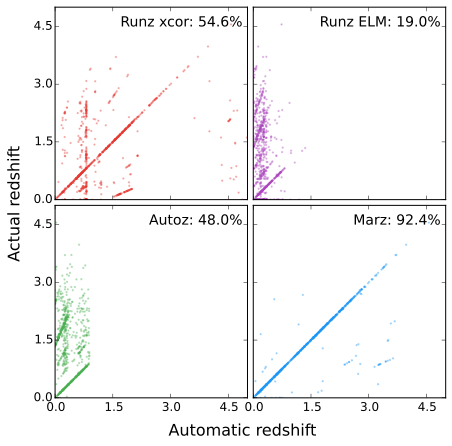
\includegraphics[width=\columnwidth]{run009Comp.png}
\caption{Low signal-to-noise, high-redshift data from the OzDES survey is used in this comparison of matching capability, with a redshift threshold of $\delta z \leq 0.01$. 1083 spectra from eight fields with a redshift range of up to 4.55 are used in this comparison. \runz{} emission line matching performs the worst, with strong diagonal lines of non-unity slope showing repeated spectra feature misidentification. Vertical banding in the \runz{} cross correlation algorithm significantly impacts its effectiveness, and \autoz{}'s lack of high redshift templates and hard-coded $z=0.9$ cutoff make the comparison almost inapplicable. Here the quasar specific matching algorithm used by \marz{} stands out, giving a success rate of over 90\% for quasar spectra.}
\label{fig:low}
\end{figure}





\section{Matching Performance}

Performance testing for \marz{} was conducted by looking at two sets of distinct data - one from the OzDES team with low signal-to-noise data at high redshift, and one from the 2dFLenS team with high signal-to-noise data. In both cases, manual redshifting was performed by experienced redshifters in \runz{}, and the automatic matches produced by \runz{} and the automatic results returned by \marz{} were compared to the manually assigned redshift for all results assigned a QOP of 4 (99\% confidence interval). Comparisons were also made with the \autoz{} program, which is the software being used for the GAMA survey and also being adopted by the 2dFLenS team. These surveys have a smaller number of object types and smaller redshift ranges than OzDES, and therefore have simpler requirements for the redshifting software. These high and low signal-to-noise results are shown in Figures \ref{fig:high} and \ref{fig:low}. The redshifting accuracy of \marz{} for high signal-to-noise data gave the correct redshift for 97.4\% of QOP4 spectra, a failure rate far less than that offered by \runz{} and comparable to \autoz{}. For the low signal-to-noise (high redshift) OzDES data, the accuracy of \marz{} was $\approx 92$\%. This is in comparison to the best \runz{} algorithm giving a total accuracy of 54.6\%. The lower success rate of \autoz, 48.0\%, is because the redshift ranges and object types found in the OzDES data are outside the matching capacity of the program.\\

In addition to the QOP4 successful recovery rates, a normalised probability distribution of likelihood for spectral line misclassification can been produced by combining the high and low signal-to-noise data, where the probability for a misclassification per correct classification can be inspected. This has been done for QOP 4 and QOP 3 (90\% confidence) results, in Figure \ref{fig:f4}. Commonly misidentified spectral lines are labelled in the figure, and can be seen to be a primary source of misclassification across al algorithms. The common [O$_{\mathrm{II}}$]/[O$_{\mathrm{III}}$] misclassification is strongly present in the \marz{} failure rates, however its significant drops to approximately 10\% of the total failure rate when only QOP4 misclassifications are considered, with the majority of the total failure rate of 4.1\% centered around 1. Whilst the expected failure rate for QOP 3 redshifts is ten times higher than for QOP 4 values, this still warrants extra investigation and potential down weighting of high redshift O$_{\rm{II}}$ matches. Commonly misclassified features are also visible on Figure \ref{fig:high} and \ref{fig:low} as linear relationships off the diagonal.\\








\begin{figure}[h]
\centering
\includegraphics[width=\columnwidth]{errorRateqop3.png}
\caption{The percentage chance, per successfully assigned redshift of quality 3 or 4, of assigning an incorrect redshift $z_A$ with respect to correct manual redshift $z_M$. Peaks in the probability distribution generally represent misidentified spectral lines, and common misidentification ratios have had the corresponding spectral lines labelled, such that the first label, MgII/H$\alpha$ represents the MgII feature misidentified as H$\alpha$ instead. Performance for \runz{} cross correlation, \runz{} emission line matching, \autoz{} and \marz{} are shown respectively in panels (a), (b), (c) and (d). Panel probability axes are not scale with one another, and the area covered represents the total failure rate. The 2dFLenS and OzDES data from Figures \ref{fig:low} and \ref{fig:high} are combined in this analysis, and QOP3 spectra (90\% confidence interval) have been included to give a greater number of sample points. The high relative failure rate of \marz{} around 1 are due to broad line matches which are not as well constrained as emission line spectrum. The total failure rates are given as follows: \runz{} cross correlation: 37.5\%, \runz{} emission line matching: 71.0\% failure rate, \autoz{}: 18.6\% failure rate, \marz{}: 6.9\% failure rate.}
\label{fig:f4}
\end{figure}











\section{Interactive Interface}

The interactive interface consists currently five primary screens: the overview, detailed, templates, settings, and usage screen. The first two screens - the overview and detailed screens, are where users will spend the vast majority of their time, and thus screenshots of them have been provided in Figures \ref{fig:overview} and \ref{fig:detailed}. The overview screen provides users with a high level view of the spectra in the loaded FITs file, detailing what they have been matched to and the quality assigned to the matches. Filtering for this screen allows users to sort results or to filter by categories, for example only displaying matches of quality (QOP) 4 or all matches to quasar templates. Comma-separated variable (CSV) output in the form of previously downloaded \marz{} results files can be loaded into the program in the same drag-and-drop manner as FITS files, allowing easy verification of redshift results by different users on different machines. A progress bar at the top of the screen keep track of current file completion and file quality.\\

The detailed screen allows for better verification of automatic matches and also offers the possibility of manually redshifting spectra. Verification of the on screen displayed redshift is done simply by assigning a QOP value, and the top five automatic matches can be cycled if the best match is visibly incorrect. Keyboard shortcuts are available for almost all actions, where key mappings are based off the shortcuts available in \runz{} in order to make transitioning from \runz{} to the \marz{} as easy as possible. Users can click on features in the detailed plot and then mark them as spectral lines. Matches can be updated by by automatically fitting to the best cross correlation value within a small deviation window. The user can also toggle whether to the display the raw data or the preprocessed data, whether to render a template under the data plot, and whether to display continuum or not. Boxcar smoothing is available to help spectrum legibility.\\

The templates screen is mostly non-interactive, and simply displays all the templates used by the system with the option to enable or disable specific templates at will. The settings screen gives options to explicitly set how many processing threads to create, whether results should be saved in the background, and offers the ability to clear all saved results in the system, or to simply clear results for the currently loaded FITs. The usage page gives instructions on how to use the program, an explanation of the purpose of each screen, how to raise issues or feature requests via GitHub, and provides several example FITs files for users who simply want to test out the system without having to source a FITs file themselves. It also provides a list of keyboard shortcuts for those users whom are not familiar with \runz{}.

Two main error safeguards have been implemented in the program to stop unnecessary loss of work. The first is a confirmation request when attempting to close down the application, which solves the issue of closing the whole browser with an open tab of \marz{}. The second and more robust solution is to use the local storage capacity available in modern browsers to save results in the background after every automatic or manual redshift is assigned. This allows users to close the program, and resume where they left off simply by dragging the original FITS file back into the application.

\begin{figure*}[H]
\centering
\includegraphics[width=\textwidth]{InterfaceZ.png}
\caption{The overview screen, showing data from a FITs file courtesy of Chris Blake and the 2dFLenS survey. Users can switch between a sortable tabular view and a graphic tile view, filter on object types, redshift ranges, templates and QOP values. The top of the screen shows the navigation menu, file completion progress bar and input for user initials. Visible at the bottom of the screen is the application footer, which shows the program's progress through automatic matching (automatically matched templates are shown in red in the graphical tiles). The bar changes colour depending on progress - green for preprocessing, red for matching and blue for completed. During the first two stages, a pause button is available to the user. If any results exist, a download button is available, which saves the current results to the file system.}
\label{fig:overview}
\end{figure*}

\begin{figure*}[H]
\centering
\includegraphics[width=\textwidth]{InterfaceZ2.png}
\caption{The detailed matching screen, showing spectrum 7 seen in the Overview screen in Figure \ref{fig:overview}. The menus at the top of the page allow the user to toggle data on or off (variance, sky spectrum, templates and whether to use the raw data or processed data). The menu bar also allows the user to reset to automatic or manual results, smooth the data, select which template to compare against, toggle between the best five automatic results, change the visual offset of the template and manually set the displayed redshift. The user can mark spectral lines by selecting a feature in the plot (either in the main plot or in any callout window) and then select the desired transition (either via keyboard shortcut or by selecting an option in the bottom row of the menu). Users can also change redshift by clicking on peaks in the cross correlation graph found between the spectra plot and the menu bars. Quality values for redshifts can also be assigned via keyboard shortcuts or via the vertical button menu on the left, and assigning a quality saves the result in the background and moves to the next spectra. In the case where the ``QOP 0 only" option is selected in the left hand bar, the user is taken to the next spectra without a quality flag set, or else it simply takes them to the next spectra ordered by ID.}
\label{fig:detailed}
\end{figure*}












\section{Conclusion}

Overall, it can be seen that for both high and low signal-to-noise data, \marz{} outperforms \runz{} on automatic matching of spectra. \marz{} also provides an enhanced and more intuitive user experience, and the web-based nature of the application means that installation and updating are now no longer of any concern at all. As such, I believe \marz{} presents a viable alternative to the \runz{} application, and a large step forward in the demonstration of web frameworks as a platform for non-intensive computational analysis.

\section*{Acknowledgements}
I would like to thank my supervisors, Tamara Davis and Chris Lidmin for their assistance throughout this project. I would also like to thank Karl Glazebrook, Chris Blake, Geraint Lewis, Fang Yuan and the rest of the OzDES and 2dFLenS teams for their feedback, input and user testing. The \marz{} tempalte catalogue comes from the WiggleZ and SDSS template samples, and multiple external libraries have been utilised in the creation of this application: Google's AngularJS, Twitter's Bootstrap, AngularUI, Armit Kapadia's fitsjs, Corban Brook's Digital Signal Processing package, Eli Grey's FileSaver.js, Tom Alexander's regression.js package, lodash and jQuery. {\green ask Tam how approrpriate it is for me to write like this if we are all authors. is it normal to still write first person?}

\bibliography{bibliography}


\end{document}

